\chapter{Multi-layer Perceptron}

\begin{multicols}{2}

\section{Integration Functions}

\noindent In perceptron, we use a simple summation for integration function:
$$u_j = \sum_{i=1}^I w_{ji}x_i - \theta_j$$

\noindent where $w_ji$ is read as the weight from $i$-th input to $j$-th neuron. \\

\noindent Quadratic integration function:
$$u_j = \sum_{i=1}^I w_{ji}x_i^2 - \theta_j$$

\noindent Spherical integration function:
$$u_j = \sum_{i=1}^I ( x_i - w_{ji})^2 - \theta_j$$

\section{Activation Functions}

\noindent We have seen the hard-limit / threshold activation function in perceptron:
$$
f(u) = 
\begin{cases}
1 & u \ge 0\\
-1 & u < 0
\end{cases}
$$

\noindent We also seen the linear activation function in perceptron:
$$f(u) = u$$

\noindent Unipolar sigmoid acivation function:
$$f(u) = \frac{1}{1+e^{-\lambda u}}$$

\noindent We get sigmoid function when $\lambda=1$

\section{Backpropagration Algorithm}

\begin{center}
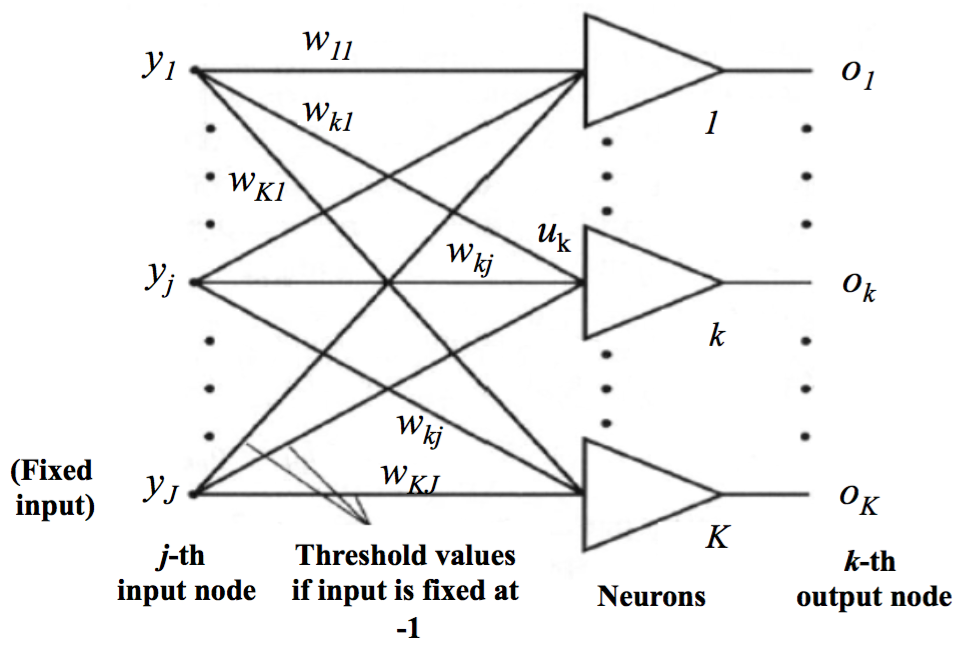
\includegraphics[width=5cm, height=5cm]{mlp}
\end{center}

\noindent The learning equation:
$$w_{kj} = w_{kj} + \lambda (d_k - o_k) .* f_k^{'}(u_k) y_j$$
$$w_{kj} = w_{kj} + \lambda \delta_{ok} .* f_k^{'}(u_k) y_j$$

\noindent Rewritten the learning equation in matrix form:
$$\mathbf{W^{new}} = \mathbf{W^{old}} + \lambda (\mathbf{d}-\mathbf{o}).* \textbf{f'(u)} \mathbf{y}^T$$

\noindent where $d$ is desired outputs and $o$ is predicted outputs. $\delta_{ok}$ is read as the error signal term for output (o) layer for $k$-neuron (the neuron in the output layer). 

\begin{center}
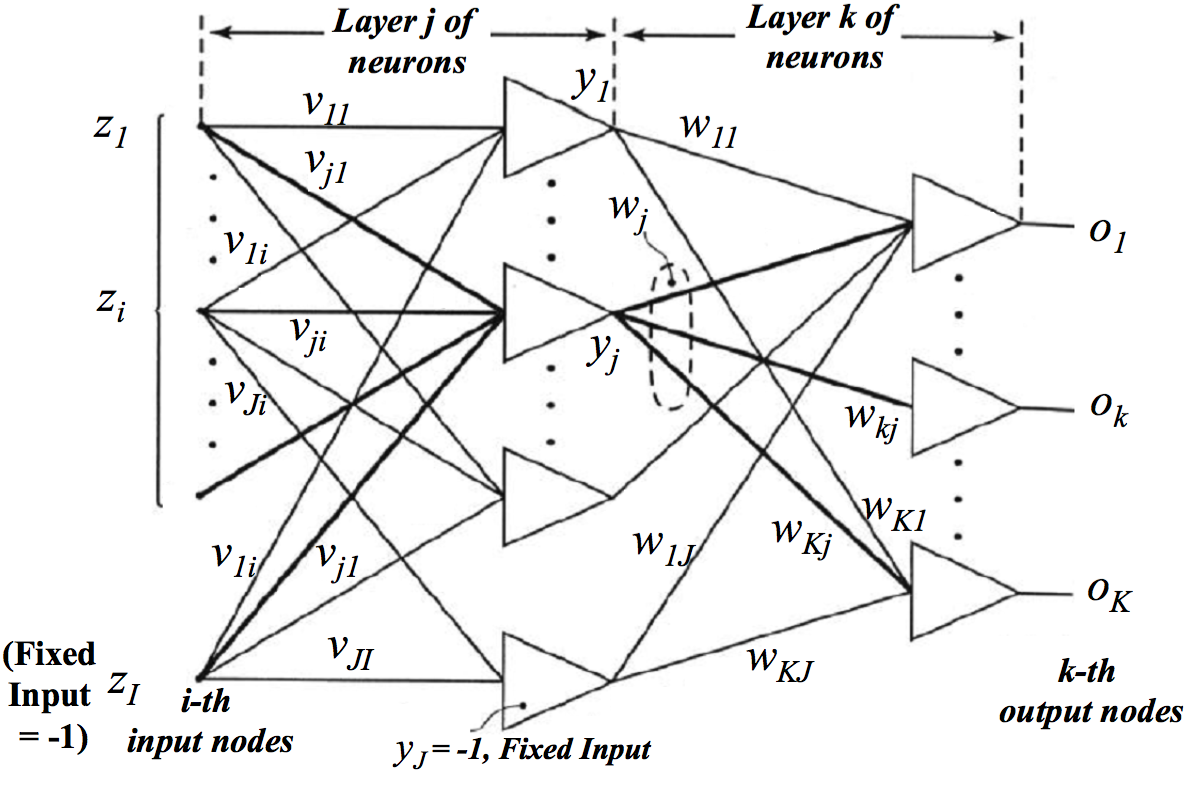
\includegraphics[width=5cm, height=5cm]{mlp_2}
\end{center}

\noindent The learning equation:
$$v_{ji}^{new} = v_{ji}^{old} + \beta \delta_{yj} z_i$$
$$\delta_{yj} = f_j'(s_j)\sum_{k=1}^{K} \delta_{ok} w_{kj}$$

\noindent Rewritten the learning equation in matrix form:
$$\mathbf{V^{new} = V^{old}} + \beta \mathbf{\delta_y z^{T}}$$
$$\mathbf{\delta_y = f'(s) .* W^{T} \delta_o}$$

\end{multicols}